\documentclass[12pt,a4paper]{article}
\usepackage[utf8]{inputenc}
\usepackage[english]{babel}
\usepackage{booktabs}
\usepackage{amsmath}
\usepackage{geometry}
\usepackage{tikz}
\usetikzlibrary{automata, positioning, arrows.meta, shapes.geometric}

\geometry{margin=2.5cm}

\title{All About State Machines: The Smart Traffic Light}
\date{2026/05/11}

\begin{document}

\maketitle

\section{What are Finite State Machines?}
Imagine a toy that has different "moods." A robot dog, for example, can "Sleep," "Bark," or "Run." But it can never do everything at the same time. This is called a \textbf{Finite State Machine (FSM)}.
\begin{itemize}
    \item \textbf{Finite} means: There is a fixed number of moods (states). It cannot suddenly do something completely unknown.
    \item \textbf{State} means: What the machine is doing right now.
\end{itemize}

\section{Describing Machines: State Chart Diagrams}
To understand how the robot thinks, we draw a \textbf{State Chart Diagram}. It is like a map with cities and roads.
\begin{itemize}
    \item \textbf{Circles (Nodes):} These are the \textbf{states} (e.g., "Light is Red"). They are the basic elements representing a specific condition.
    \item \textbf{Arrows (Edges):} These are the \textbf{transitions} or paths from one state to the next.
    \item \textbf{Events (Inputs):} This is the text written on the arrows. it is the reason why the machine moves (e.g., "Button pressed").
\end{itemize}

\section{Moore vs. Mealy: Two Types of Robots}
There are two main ways machines handle their tasks:
\begin{enumerate}
    \item \textbf{Moore Machine:} The machine only looks at its current mood. If it is in the "Happy" state, it laughs. It doesn't matter what is happening outside at that exact moment. The \textbf{output depends only on the state}.
    \item \textbf{Mealy Machine:} This machine reacts faster. It laughs only if it is in the "Happy" state \textbf{and} someone tells a joke at the same time. The \textbf{output depends on both the state and the input}.
\end{enumerate}

\section{The Traffic Light Example}
Here, our machine controls a traffic light for cars that reacts to a pedestrian button ($X$).

\subsection{State Chart Diagram}
\begin{figure}[h]
\centering
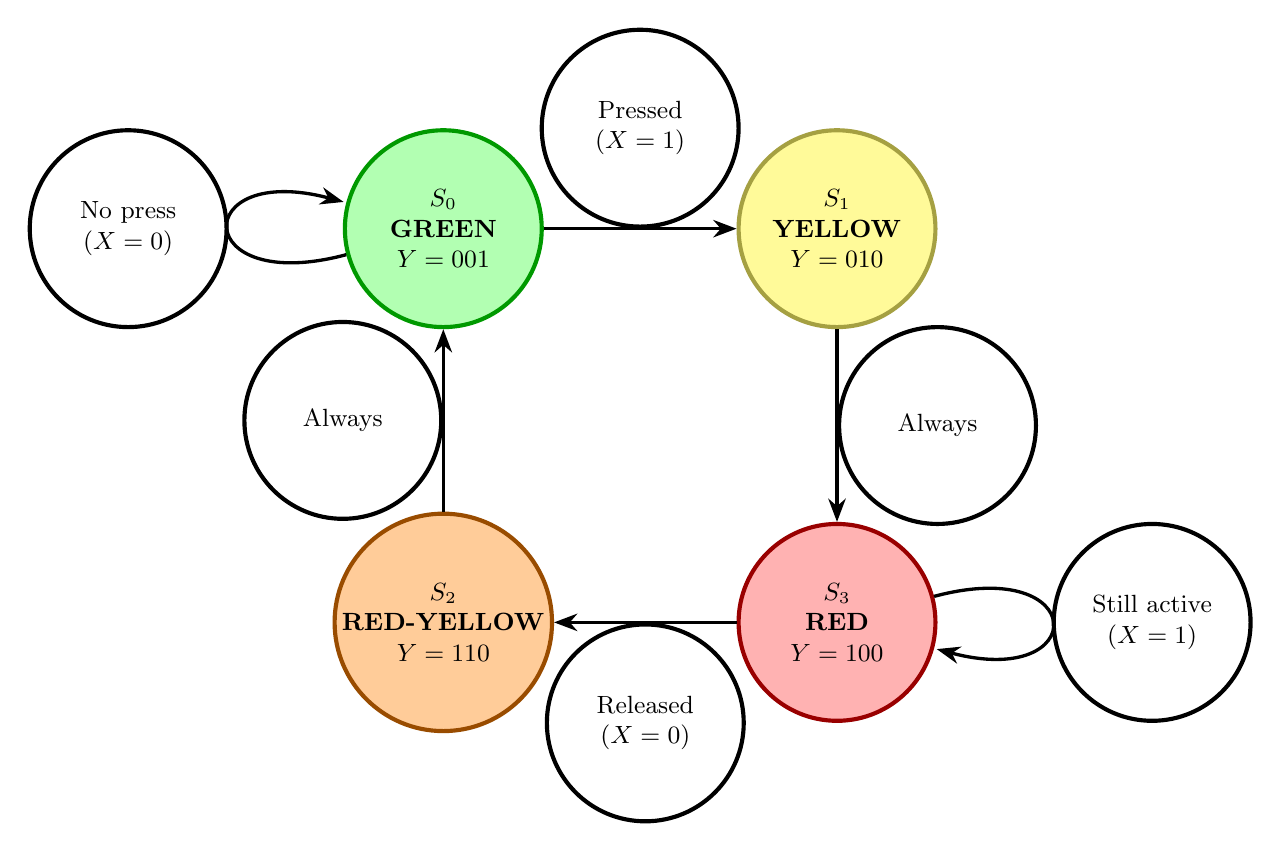
\begin{tikzpicture}[->, >=Stealth, node distance=5cm, 
    every node/.style={
        circle, 
        draw, 
        minimum size=2.5cm, 
        inner sep=0pt, 
        align=center, 
        line width=1.5pt, 
        font=\small
    }]

    % States with uniform diameter and traffic light colors
    \node[fill=green!30, draw=green!60!black] (S0) {$S_0$ \\ \textbf{GREEN} \\ $Y=001$};
    \node[fill=yellow!40, draw=yellow!60!black] (S1) [right of=S0] {$S_1$ \\ \textbf{YELLOW} \\ $Y=010$};
    \node[fill=red!30, draw=red!60!black] (S3) [below of=S1] {$S_3$ \\ \textbf{RED} \\ $Y=100$};
    \node[fill=orange!40, draw=orange!60!black] (S2) [below of=S0] {$S_2$ \\ \textbf{RED-YELLOW} \\ $Y=110$};

    % Transitions
    \path[line width=1.2pt]
        (S0) edge [loop left] node {No press \\ ($X=0$)} (S0)
        (S0) edge node [above] {Pressed \\ ($X=1$)} (S1)
        (S1) edge node [right] {Always} (S3)
        (S3) edge [loop right] node {Still active \\ ($X=1$)} (S3)
        (S3) edge node [below] {Released \\ ($X=0$)} (S2)
        (S2) edge node [left] {Always} (S0);
\end{tikzpicture}
\caption{Moore state machine for traffic light control[cite: 30, 36].}
\end{figure}

\newpage
\section{Implementing the Moore Machine}
To build the machine, we fill in two functional tables.

\subsection{1. Transient Functions (Transitions)}
This table tells us: "If I am here and this happens, I go there."

\begin{table}[h]
\centering
\begin{tabular}{lcll}
\toprule
Current State & Input (Button $X$) & Next State & Explanation \\
\midrule
$S_0$ (Green) & 0 & $S_0$ & No one presses, stays Green. \\
$S_0$ (Green) & 1 & $S_1$ & Someone presses, turns Yellow. \\
$S_1$ (Yellow) & 0 or 1 & $S_3$ & Yellow always turns to Red. \\
$S_3$ (Red) & 1 & $S_3$ & Stays Red as long as pressed. \\
$S_3$ (Red) & 0 & $S_2$ & Button released, preparation. \\
$S_2$ (Red-Yellow) & 0 or 1 & $S_0$ & Back to start (Green). \\
\bottomrule
\end{tabular}
\end{table}

\subsection{2. Output Functions}
This table tells us: "In this state, these lights turn on." ($y_2$=Red, $y_1$=Yellow, $y_0$=Green).

\begin{table}[h]
\centering
\begin{tabular}{lccl}
\toprule
State & Code ($y_2 y_1 y_0$) & Light Signal & What does the car see? \\
\midrule
$S_0$ & 001 & Green & Driving allowed. \\
$S_1$ & 010 & Yellow & Caution, stop soon. \\
$S_2$ & 110 & Red + Yellow & Caution, starting soon. \\
$S_3$ & 100 & Red & Stop! \\
\bottomrule
\end{tabular}
\end{table}

\end{document}